\documentclass[a4paper,12pt]{article}
%For images
\usepackage{graphicx}
 
\addtolength{\oddsidemargin}{-.875in}
\addtolength{\evensidemargin}{-.875in}
\addtolength{\textwidth}{1.75in}
 
\addtolength{\topmargin}{-.875in}
\addtolength{\textheight}{1.75in}
 
\begin{document}
\begin{enumerate}
    \item Man flippar den upp och ner samt spegelvänd:

          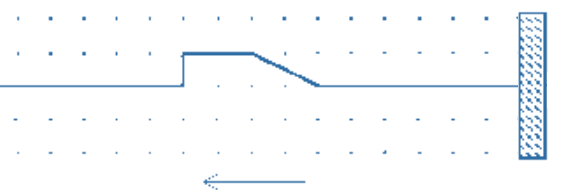
\includegraphics{Figur 1.png}

    \item
          I det slutna röret så kommer sju noder att skapas,
          vilket är toppar och dalar vilket bildar följande bild:
          \begin{center}
              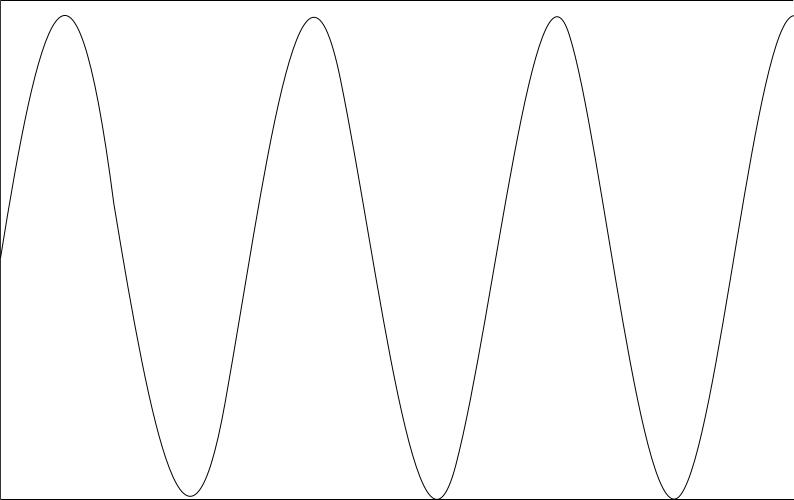
\includegraphics[scale=0.5]{Figur 2.png}
          \end{center}

          Vi kan observera att antalet våglängder som passerar
          är 13/4. Då får vi från ekvationerna att längden L är
          likamed 13/4 gånger våglängden $\lambda$.

          $$L=\frac{13}{4}\lambda \Rightarrow \lambda=L\frac{4}{13}$$

          Med hastighetsekvationen blir det

          $$v=f\lambda=fL\frac{4}{13}=870\cdot 1.5\cdot \frac{4}{13}\approx 402m/s$$

          Detta är ett väldigt rimligt tal då det är nära hastigheten
          för ljudet i luften som är 343 m/s.

    \item Med brytningslagen får vi
          $$v_2\sin(\alpha)=v_1\sin(90)\Rightarrow v_2\sin(\alpha)=v_1$$
          Då utfallsvinkeln är 90 grader för att det är en rätvinkel
          och då måste $\alpha$ bli gränsvinkeln.
          $$\alpha = \sin^{-1}(\frac{v_1}{v_2})=\sin^{-1}(\frac{340}{1490})\approx 13.2^\circ$$

    \item Jag fyllde ett glas med vatten och lade i en penna snett i vattnet.
          Sedan mättes olika längder för att ta fram vinklarna

          $$\tan(i)=\frac{6}{5}$$
          $$\tan(b)=\frac{7}{10}$$

          brytningslagen med luft är $n\sin(i)=\sin(b)$
          Då följer det att
          $$\sin(\tan^{-1}(\frac{6}{5}))=n\sin(\tan^{-1}(\frac{7}{10}))\Rightarrow n=\frac{\sin(\tan^{-1}(\frac{7}{10})}{\sin(\tan^{-1}(\frac{6}{5}))}\approx 1.33$$

    \item Med gitterformeln
          $$d\sin(\alpha)=n\lambda\Rightarrow \lambda=\frac{d\sin(\alpha)}{n}$$

          Med värderna i uppgiften är

          $d=1.67\cdot 10^{-6}$,

          $n=2$ för att de är mellan det yttre, andragradens strålarna vinkeln mäts,

          $\alpha = 94.1/2 = 47.05$ Eftersom att vinkeln från centralstrålen till en ytterstråle är halva vinkeln
          mellan de två yttre strålarna.

          Våglängden och svaret på uppgiften blir då
          $$\lambda=\frac{1.67\cdot 10^{-6}{\sin(47.05)}}{2}\approx 6.1118\cdot 10^{-7}$$
          dvs våglängden är 611 nm.

    \item Ljudnivån defineras som $L=10\lg(\frac{I}{I_0})$ där $I_0$ då är en jämförelseenhet
          som kan ignoreras då den är lika med 1 och $I=\frac{W}{m^2}$ . I uppgiften får vi reda på att
          ljudstyrkan 10 meter från stället är 110, då kan man derivera kraften som
          jetmotorn ger ut.

          $$L_0=110=10\lg(\frac{W}{10^2})\Rightarrow 100\cdot 10^{11}=10^{13}=W$$

          Då sätter vi in W då jeymotorn fortsätter ha samma kraft, medans vi räknar med antalet meter som 1000

          $$L_1=10\lg(\frac{10^{13}}{1000^2})=10\lg(\frac{10^{13}}{10^6})=10\cdot 7 = 70db$$

          Ljudet uppmäts alltså som 70 decibel när man står 1 km från flygplanet.

    \item I uppgiften så får vi värderna som behövs för att räkna ut gitterkonstanten

          $$d=\frac{n_1\lambda_1}{\sin(\alpha_1)}$$

          Där $n_1=3$ eftersom det går till tredje ordningens ljus,
          $\lambda_1=5.893\cdot 10^{-7}$ och $\alpha=105.4/2=52.7$ då
          man räknar vinkeln mellan centralstrålen och den yttersta strålen.

          $$d=\frac{3\cdot 5.893\cdot 10^{-7}}{\sin(52.7)}\approx 2.22\cdot 10^{-6}$$

          Med det blir nya värden med den nya lasern. $\lambda_2=4.35\cdot 10^{-7}$ och
          där den maximala vinkeln $\alpha=90$. Vi löser ut för $n_2$:

          $$n_2=\frac{d\sin(\alpha_2)}{\lambda_2}=\frac{2.22\cdot 10^{-6}\sin(90)}{4.35\cdot 10^{-7}}\approx 5.1$$

          Vilket innebär att maximala ordningens ljus är 5, så med fem på båda sidorna av centralstrålen
          samt centralstrålen blir det 11 möjliga ljuspunkter.

\end{enumerate}
\end{document}